%=============================================================================
% PREAMBUL COMUN - Statistica Piețelor Financiare
% Versiune robustă pentru macOS (MacTeX / BasicTeX / TeX Live)
% Daniel Traian Pele, Antoaneta Amza - ASE București
%
% MODIFICĂRI față de varianta originală:
%  (1) fontawesome5 făcut OPȚIONAL (\IfFileExists) → nu mai pică dacă lipsește
%  (2) polyglossia cu fallback automat pe babel dacă romanian nu există
%  (3) setmainfont rescris cu Ligatures=TeX și nume normalizate (merge pe macOS)
%  (4) graphicspath extins (include directorul curent + variante relative) ca
%      logo-urile să fie găsite și când lansezi xelatex dintr-un subdirector
%
% Compilare:  xelatex preamble + main, de DOUĂ ori (toc/ref).
%=============================================================================

% Asigură încadrarea conținutului pe diapozitive
\setbeamersize{text margin left=8mm, text margin right=8mm}

%=============================================================================
% CONFIGURARE TEMĂ ȘI STIL
%=============================================================================
\usetheme{default}

% Paletă de Culori
\definecolor{MainBlue}{RGB}{26, 58, 110}
\definecolor{AccentBlue}{RGB}{26, 58, 110}
\definecolor{IDAred}{RGB}{205, 0, 0}
\definecolor{DarkGray}{RGB}{51, 51, 51}
\definecolor{MediumGray}{RGB}{128, 128, 128}
\definecolor{LightGray}{RGB}{248, 248, 248}
\definecolor{VeryLightGray}{RGB}{235, 235, 235}
\definecolor{KeynoteGray}{RGB}{218, 218, 218}
\definecolor{SectionGray}{RGB}{120, 120, 120}
\definecolor{FooterGray}{RGB}{100, 100, 100}
\definecolor{Crimson}{RGB}{220, 53, 69}
\definecolor{Forest}{RGB}{46, 125, 50}
\definecolor{Amber}{RGB}{181, 133, 63}
\definecolor{Orange}{RGB}{230, 126, 34}
\definecolor{Purple}{RGB}{142, 68, 173}

% Fundal gradient (gradient Keynote exact 315°: alb la RGB 218,218,218)
\setbeamertemplate{background}{%
	\begin{tikzpicture}[remember picture, overlay]
		\shade[shading=axis, shading angle=315,
		top color=white, bottom color=KeynoteGray]
		(current page.south west) rectangle (current page.north east);
	\end{tikzpicture}%
}
% Culoare solidă de rezervă pentru compatibilitate
\setbeamercolor{background canvas}{bg=}

\setbeamercolor{palette primary}{bg=MainBlue, fg=white}
\setbeamercolor{palette secondary}{bg=MainBlue!85, fg=white}
\setbeamercolor{palette tertiary}{bg=MainBlue!70, fg=white}
\setbeamercolor{structure}{fg=MainBlue}
\setbeamercolor{title}{fg=IDAred}
\setbeamercolor{frametitle}{fg=IDAred, bg=}
\setbeamercolor{block title}{bg=MainBlue, fg=white}
\setbeamercolor{block body}{bg=VeryLightGray, fg=DarkGray}
\setbeamercolor{block title alerted}{bg=Crimson, fg=white}
\setbeamercolor{block body alerted}{bg=Crimson!8, fg=DarkGray}
\setbeamercolor{block title example}{bg=Forest, fg=white}
\setbeamercolor{block body example}{bg=Forest!8, fg=DarkGray}
\setbeamercolor{item}{fg=MainBlue}

\setbeamerfont{institute}{size=\footnotesize}

\setbeamercolor{author in head/foot}{fg=FooterGray, bg=}
\setbeamercolor{title in head/foot}{fg=FooterGray, bg=}
\setbeamercolor{date in head/foot}{fg=FooterGray, bg=}
\setbeamercolor{section in head/foot}{fg=FooterGray, bg=}
\setbeamercolor{subsection in head/foot}{fg=FooterGray, bg=}

\setbeamertemplate{itemize item}{\color{MainBlue}$\boxdot$}
\setbeamertemplate{itemize subitem}{\color{MainBlue}$\blacktriangleright$}
\setbeamertemplate{itemize subsubitem}{\color{MainBlue}\tiny$\bullet$}
\setbeamertemplate{itemize/enumerate body begin}{\normalsize}
\setbeamertemplate{itemize/enumerate subbody begin}{\normalsize}

\setbeamertemplate{section in toc}{%
	\leavevmode\leftskip=1.5em%
	\llap{\color{MainBlue}$\boxdot$\kern0.5em}%
	\inserttocsection\par%
}

\setlength{\leftmargini}{10pt}
\setlength{\leftmarginii}{10pt}
\makeatletter
\def\@listi{\leftmargin\leftmargini \topsep 0pt \parsep 0pt \itemsep 0pt}
\def\@listii{\leftmargin\leftmarginii \topsep 0pt \parsep 0pt \itemsep 0pt}
\makeatother

\setbeamertemplate{navigation symbols}{}

%=============================================================================
% ANTET PERSONALIZAT
%=============================================================================
\setbeamertemplate{headline}{%
	\vskip10pt%
	\hbox to \paperwidth{%
		\hskip0.5cm%
		{\small\color{FooterGray}\renewcommand{\hyperlink}[2]{##2}\insertsectionhead}%
		\hfill%
		\textcolor{FooterGray}{\small\insertframenumber}%
		\hskip0.5cm%
	}%
	\vskip4pt%
	{\color{FooterGray}\hrule height 0.4pt}%
}

%=============================================================================
% PACHETE — ordine importantă: fontspec ÎNAINTE de polyglossia/babel
%=============================================================================

% --- (1) FONTSPEC + FONTURI ROBUSTE PE macOS ---
\usepackage{fontspec}
% Pe macOS unele fonturi Latin Modern nu sunt înregistrate ca fonturi de sistem.
% Folosim Ligatures=TeX (pentru -- → en-dash etc.) și lăsăm fontspec să caute
% prin kpathsea (merge atât pe Mac, cât și pe Linux/Windows).
\defaultfontfeatures{Ligatures=TeX}
\IfFontExistsTF{Latin Modern Roman}{%
	\setmainfont{Latin Modern Roman}
	\setsansfont{Latin Modern Sans}
	\setmonofont{Latin Modern Mono}
}{%
	% Fallback dacă numele cu spații nu sunt găsite (cazul macOS fără fonturi
	% Latin Modern în /Library/Fonts) — fontspec va folosi fontul implicit.
	\PackageWarning{preamble}{Latin Modern Roman nu a fost gasit; folosesc fontul implicit.}
}

% --- (2) POLYGLOSSIA SAU BABEL CU FALLBACK ---
% Pe versiuni vechi de polyglossia (TeX Live < 2020) limba `romanian` nu există.
% Detectăm și folosim babel ca rezervă.
\IfFileExists{gloss-romanian.ldf}{%
	\usepackage{polyglossia}
	\setdefaultlanguage{romanian}
	\setotherlanguage{english}
}{%
	\PackageWarning{preamble}{polyglossia/romanian indisponibil; folosesc babel.}
	\usepackage[english,romanian]{babel}
}

% --- (3) MATH ȘI GRAFICĂ ---
\usepackage{amsmath, amssymb, amsthm}
\usepackage{mathtools}
\usepackage{bm}
\usepackage{tikz}
\usetikzlibrary{arrows.meta, positioning, shapes, calc, decorations.pathreplacing, shadings}
\usepackage{booktabs}
\usepackage{multirow}
\usepackage{array}
\usepackage{graphicx}
\usepackage{hyperref}
\usepackage{colortbl}
\usepackage{listings}
\lstset{basicstyle=\ttfamily\small, breaklines=true, frame=single, backgroundcolor=\color{VeryLightGray}}
\hypersetup{colorlinks=true, linkcolor=MainBlue, urlcolor=MainBlue}

% --- (4) GRAPHICSPATH cu directorul curent inclus ca fallback ---
\graphicspath{{./}{./logos/}{./charts/}{./photos/}{../logos/}{../charts/}{../photos/}{../../logos/}{../../charts/}{../../photos/}}
\hfuzz=2pt
\vfuzz=2pt

%=============================================================================
% SUBSOL PERSONALIZAT — fontawesome5 făcut OPȚIONAL
%=============================================================================
% Pe BasicTeX / instalări minime de MacTeX, fontawesome5 nu există.
% Dacă lipsește, omitem icoanele (subsolul rămâne curat).
\IfFileExists{fontawesome5.sty}{%
	\usepackage{fontawesome5}
	\newcommand{\hasfontawesome}{true}
}{%
	\PackageWarning{preamble}{fontawesome5 indisponibil; subsolul nu va contine icoane.}
}

\setbeamertemplate{footline}{%
	{\color{FooterGray}\hrule height 0.4pt}%
	\vskip4pt%
	\hbox to \paperwidth{%
		\hskip0.5cm%
		\textcolor{FooterGray}{\small Statistica Piețelor Financiare}%
		\hfill%
		\raisebox{-0.1em}{%
			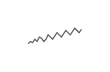
\begin{tikzpicture}[x=0.08em, y=0.08em, line width=0.4pt]
				\draw[FooterGray] (0,3) -- (1,4) -- (2,3.5) -- (3,5) -- (4,4) -- (5,6) -- (6,5.5) -- (7,4) -- (8,5) -- (9,7) -- (10,6) -- (11,5) -- (12,6.5) -- (13,8) -- (14,7) -- (15,6) -- (16,7.5) -- (17,9) -- (18,8) -- (19,7) -- (20,8.5) -- (21,10) -- (22,9) -- (23,8) -- (24,9.5);
			\end{tikzpicture}%
		}%
		\hskip0.5cm%
	}%
	\vskip6pt%
}

%=============================================================================
% COMANDA QUANTLET
%=============================================================================
\newcommand{\quantlet}[2]{%
	\hfill\href{#2}{%
		\raisebox{-0.15em}{
\includegraphics[height=0.7em]{ql_logo.png}}%
		\textcolor{MainBlue}{\tiny\ #1}%
	}%
}

%=============================================================================
% PAGINĂ TITLU PERSONALIZATĂ
%=============================================================================
\defbeamertemplate*{title page}{hybrid}[1][]
{
	\vspace{0.2cm}
	\noindent\makebox[\linewidth][s]{%
		\href{https://www.ase.ro}{
\includegraphics[height=1.0cm]{ase_logo.png}}\hfill%
		\href{https://theida.net}{
\includegraphics[height=1.0cm]{ida_logo.png}}\hfill%
		\href{https://blockchain-research-center.com}{
\includegraphics[height=1.0cm]{brc_logo.png}}\hfill%
		\href{https://www.ai4efin.ase.ro}{
\includegraphics[height=1.0cm]{ai4efin_logo.png}}\hfill%
		\href{https://ipe.ro/new}{
\includegraphics[height=1.0cm]{acad_logo.png}}\hfill%
		\href{https://www.digital-finance-msca.com}{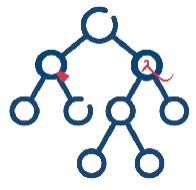
\includegraphics[height=1.0cm]{msca_logo.png}}%
	}
	\vspace{0.6cm}
	
	\noindent\makebox[\linewidth][c]{%
		\begin{minipage}{0.11\linewidth}
			\centering
			\href{https://quantlet.com}{
\includegraphics[height=1.1cm]{ql_logo.png}}
		\end{minipage}%
		\begin{minipage}{0.76\linewidth}
			\centering
			{\LARGE\bfseries\usebeamercolor[fg]{title}\inserttitle}
			
			\vspace{0.3cm}
			
			{\usebeamerfont{subtitle}\usebeamercolor[fg]{title}\insertsubtitle}
		\end{minipage}%
		\begin{minipage}{0.11\linewidth}
			\centering
			\href{https://quantinar.com}{
\includegraphics[height=1.1cm]{qr_logo.png}}
		\end{minipage}%
	}
	
	\vspace{0.6cm}
	
	\hspace{0.5cm}{\usebeamerfont{author}\insertauthor}
	
	\vspace{0.3cm}
	
	\hspace{0.5cm}\begin{minipage}[t]{0.9\textwidth}
		\raggedright\small\insertinstitute
	\end{minipage}
}
\setbeamertemplate{title page}[hybrid]

%=============================================================================
% MEDII PENTRU TEOREME
%=============================================================================
\theoremstyle{definition}
\setbeamertemplate{theorems}[numbered]
\newtheorem{defn}{Definiție}
\newtheorem{thm}{Teoremă}
\newtheorem{prop}{Propoziție}
\newtheorem{rmk}{Observație}

%=============================================================================
% CENTRED MINIPAGE
%=============================================================================
\newenvironment{cminipage}[1]{%
	\par\noindent\hfill\begin{minipage}{#1}\ignorespaces
	}{%
	\end{minipage}\hfill\null\par
}

%=============================================================================
% COMENZI PERSONALIZATE
%=============================================================================
\newcommand{\E}{\mathbb{E}}
\newcommand{\Var}{\text{Var}}
\newcommand{\Cov}{\text{Cov}}
\newcommand{\Corr}{\text{Corr}}
\newcommand{\VaR}{\text{VaR}}
\newcommand{\ES}{\text{ES}}
\newcommand{\R}{\mathbb{R}}
\newcommand{\N}{\mathbb{N}}
\newcommand{\Z}{\mathbb{Z}}
\newcommand{\B}{\mathbf{B}}
\newcommand{\imark}{\textcolor{MainBlue}{\textbullet}}
\newcommand{\RMSE}{\text{RMSE}}
\newcommand{\MAE}{\text{MAE}}
\newcommand{\MAPE}{\text{MAPE}}
\newcommand{\correct}{\textcolor{Forest}{\checkmark}}
\newcommand{\incorrect}{\textcolor{Crimson}{\texttimes}}

%=============================================================================
% INFORMAȚII TITLU
%=============================================================================
\title[Statistica Piețelor Financiare]{Statistica Piețelor Financiare}
\author[D.T. Pele, A. Amza]{\texorpdfstring{\begin{tabular}[t]{@{}l@{}}Daniel Traian PELE \\ Antoaneta Amza\end{tabular}}{Daniel Traian PELE, Antoaneta Amza}}
\institute{Academia de Studii Economice din București\\
	IDA Institute Digital Assets\\
	Blockchain Research Center\\
	AI4EFin Artificial Intelligence for Energy Finance\\
	Academia Română, Institutul de Prognoză Economică\\
	MSCA Digital Finance}
\date{}